\capitulo{6}{Trabajos relacionados}
A nivel de proyecto hemos encontrado pocas ideas que a nivel global puedan formar un asistente de visitas de museos, sin embargo se puede hacer una comparación con distintos proyectos que tienen cosas en común.

Para ello compararemos los tres proyectos de investigación que se enumeran a continuación de manera separada con las distintas prestaciones que tiene nuestra aplicación:
\begin{itemize}
    \item Este proyecto \textit{open source} simula los planos de un museo permitiendo distintas interacciones del usuario con el mapa: \url{https://github.com/arcataroger/openlayers_indoor_map}
    \item La localización \textit{indoor} mediante \textit{Wifi} suele basarse en la recolección de \textit{fingerprints} de dispositivos de los usuarios, entrenar un modelo de algún algoritmo como \textit{KNN} y que prediga las ubicaciones exactas de los usuarios, este método es vulnerable al ruido en la recoleccion de datos y suele ser preciso en cuestión de metros.\cite{wifiIndoor}
    \item La localización \textit{indoor} con \textit{Bluetooth Low Energy (BLE)} se basa en medir la potencia de señal que reciben los \textit{beacons}, dispositivos que implementan \textit{BLE}, para localizarlos. Son más vulnerables que \textit{UWB} a ruido en las señales y en base a la potencia que reciba de la señal será más o menos preciso.
\end{itemize}

Se añade una tabla resumen de las métricas teóricas de cada una de las tecnologías\cite{comparacionIndoor}:
\FloatBarrier
\tablaSmall{Tabla resumen de comparación entre tecnologías para \textit{indoor positioning}.}{l c c c c}{resume-of-tec-for-positioning}{ \multicolumn{1}{l}{Tecnología} & Precisión & Rango \\}{ 
Wifi & < 15 m & < 150 m & &\\
BLE 4 & < 8 m & < 75 m & &\\
BLE 5.1 & < 1 m & < 75 m & &\\
UWB & < 30 cm & < 150 m & &\\
}{t}
\FloatBarrier

\section{Field Museum Map}

En este proyecto podemos encontrar una implementación de un mapa con la herramienta \textit{OpenLayers}, también usada en el proyecto práctico de este TFG, y desarrollado con \textit{Angular} para una \textit{webapp}, en la cual se crean diferentes salas y se insertan distintas imágenes temáticas y figuras indicadoras de dirección, que permiten a un usuario tener una experiencia más avanzada que en una visita a un museo normal. También es interesante comentar que implementa un sistema de cambio de planta, que permite dar más dinamismo a la web que está utilizando el usuario.

Sin embargo no implementa ningún tipo de geolocalización de usuarios, ni tampoco tiene ningún tipo de interacción directa de movimiento con las capas que utiliza, pero asienta las bases para poder implementarla sobre el mapa.
\FloatBarrier

\begin{figure}
    \centering
    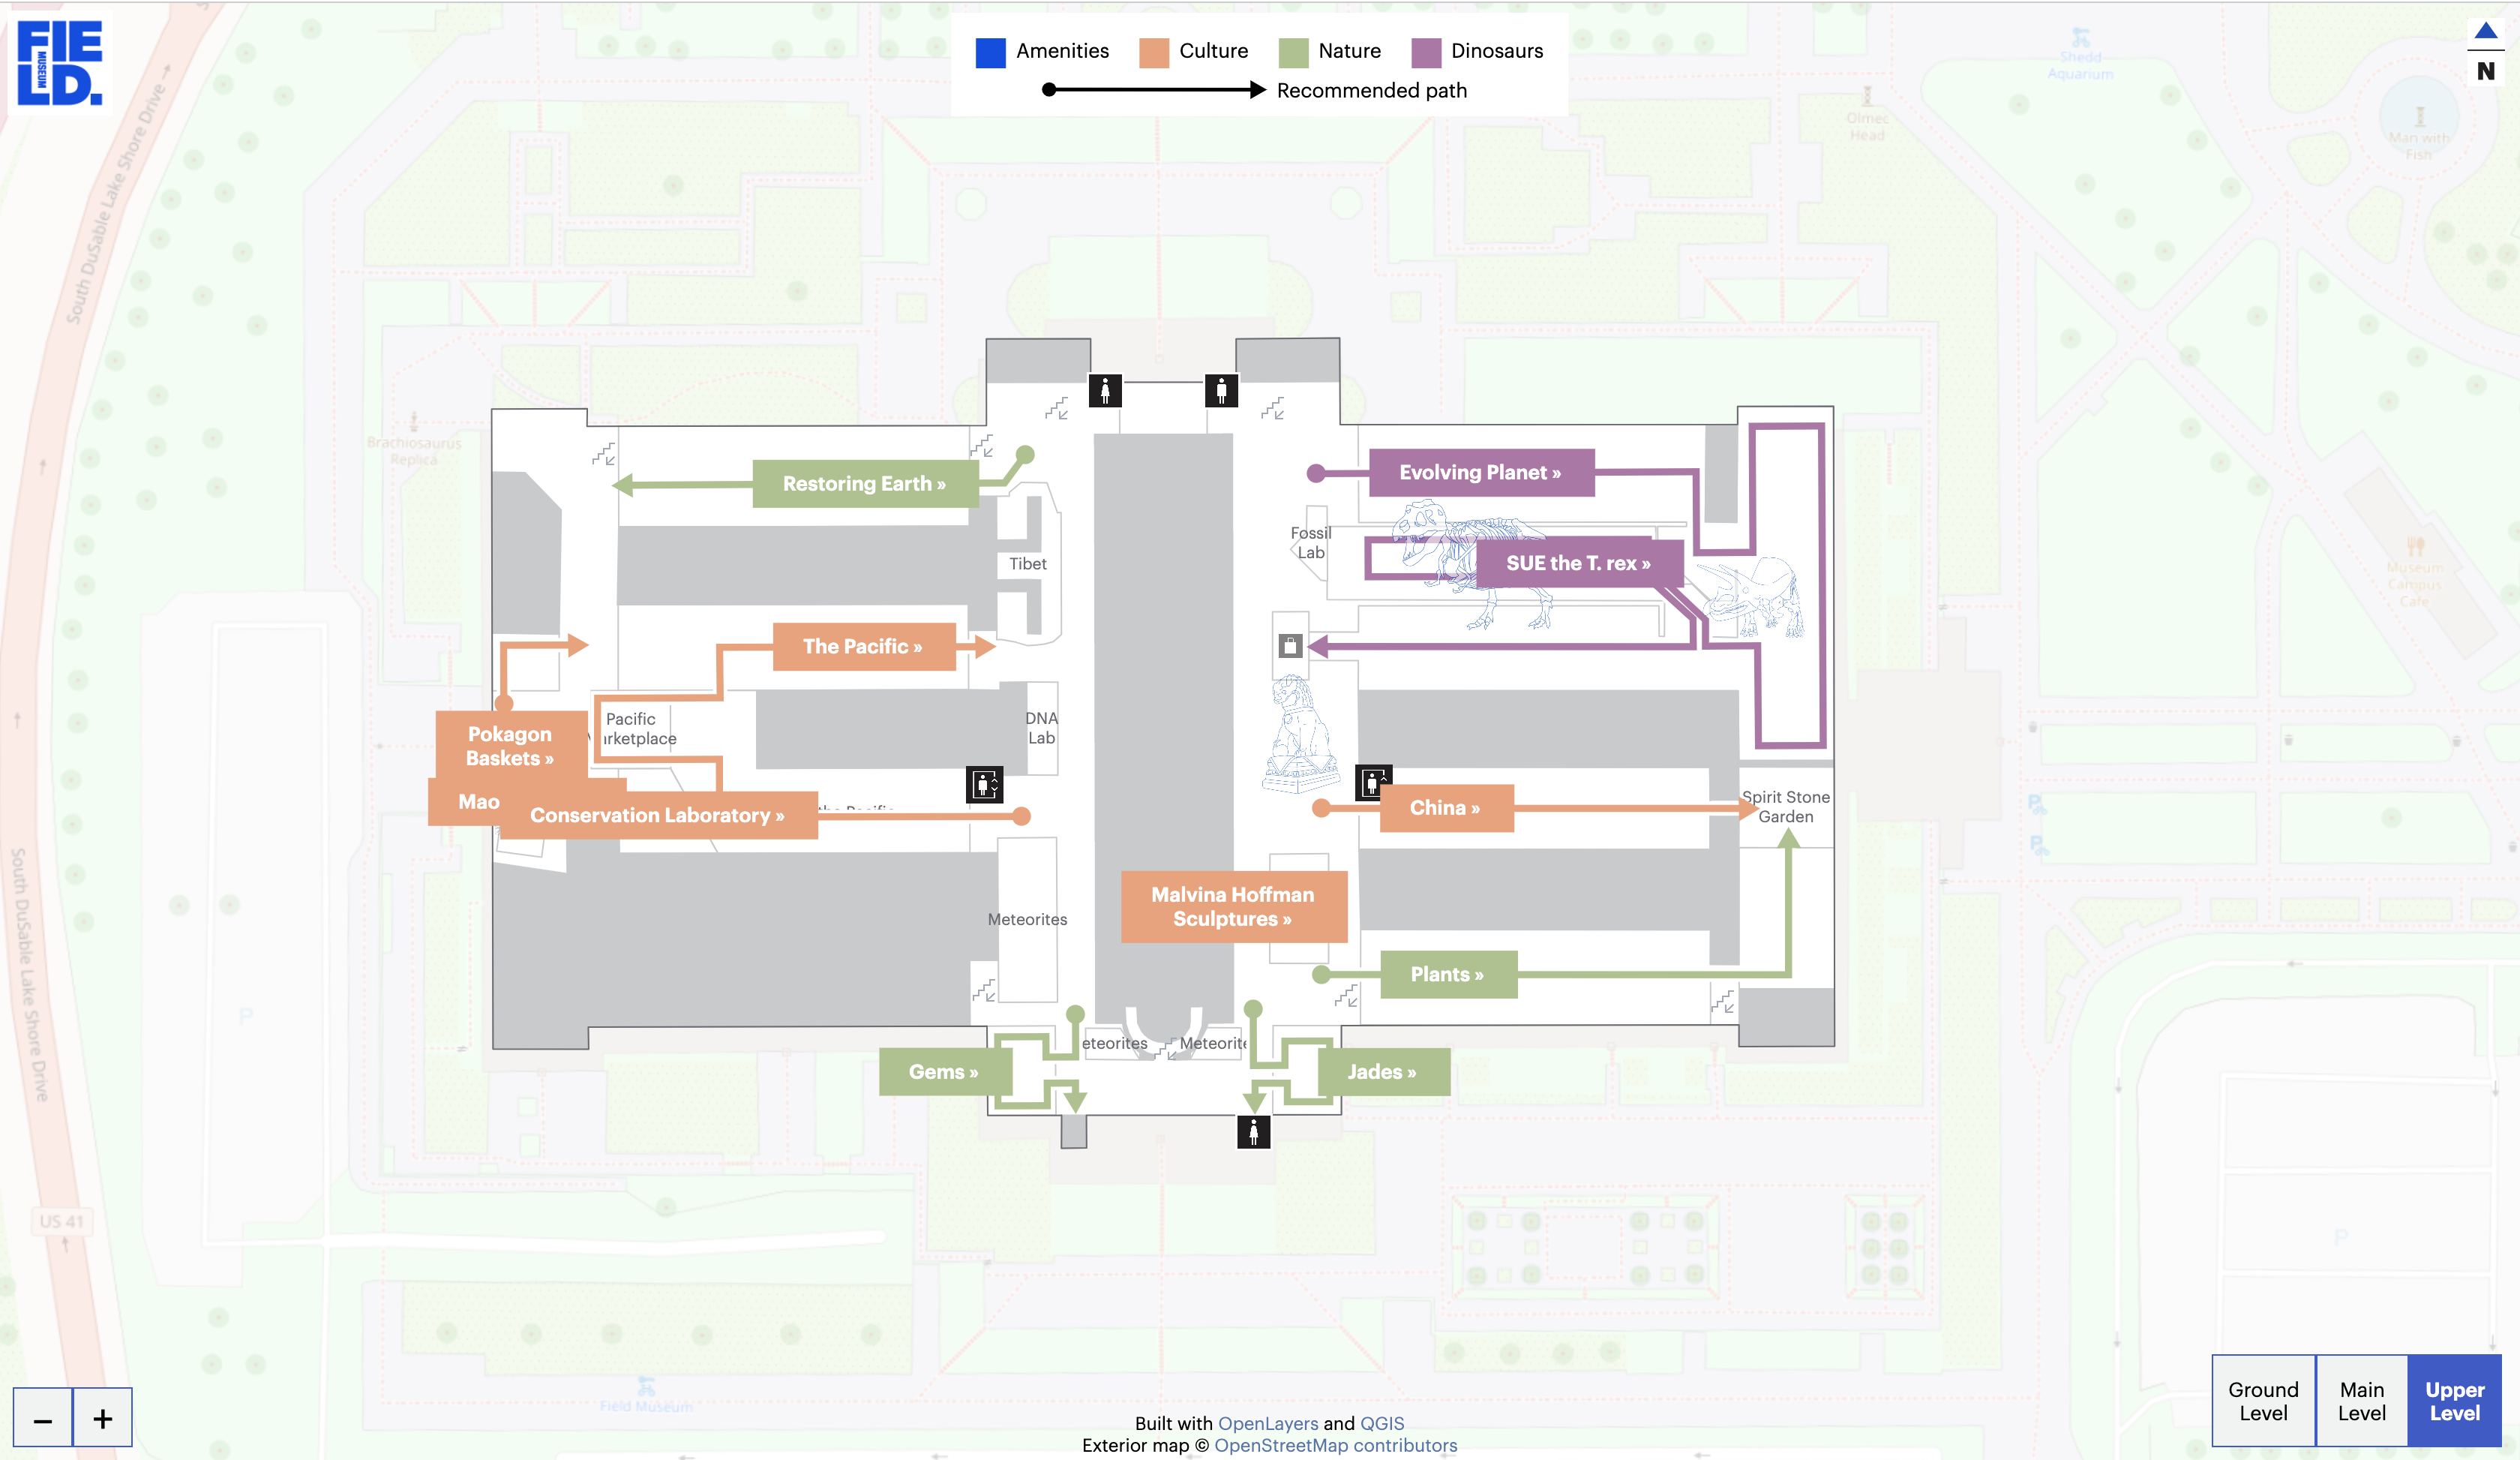
\includegraphics[width=10cm,height=10cm,keepaspectratio]{img/field_map_museum.png}
    \caption{Imagen de la Demo del proyecto \textit{Field Museum Map}.}
    \label{fig:field_museum_demo_img}
\end{figure}
\FloatBarrier

Link del proyecto: \url{https://github.com/arcataroger/openlayers_indoor_map}

Link de la Demo: \url{https://map.fieldmuseum.org/?utm_campaign=open_source&utm_source=github_readme&utm_medium=web}